\subsection{The Fano mirror: a sub wavelength grating}\label{sec:fano_mirror}

\subsubsection{Geometric optical analysis}

Considering an ideal grating with period \emph{d} in the sub-wavelength regime, it can be shown that only a single mode of reflection/transmission is supported. 

Any grating, of arbitrary dimensions, must comply with the very general \emph{grating equation}\cite{Pedrotti} given as
\begin{equation}
    \sin \theta_m = m \frac{\lambda}{d},
\end{equation}
for the special case of a linearly polarized plane wave incident on a grating placed normal to the direction of propagation. Now, inserting the sub-wavelength condition \emph{d << $\lambda$}, it is easily seen that the right side of the equation blows up for any order of reflection $|m| > 0$, effectively showing that this is the aforementioned single supported mode in this regime. Furthermore, it can be equally easily seen that the propagation direction of the 0'th order mode is the same as the incident beam, i.e. normal to the grating.

\subsubsection{Reflection/transmission spectra and line shape analysis}

\subsubsection{Lossless grating}

We wish to analytically describe the wavelength-dependent spectra for the transmission and reflectivity of an infinite sub-wavelength grating. By first considering the case where absorption and thermal coupling effects are neglected, i.e. a lossless grating, we can assume conservation of energy and thereby the relations
\begin{equation}
    |r_g|^2+|t_g|^2=1 \hspace{0.5cm} \text{and} \hspace{0.5cm} |r_d|^2+|t_d|^2=1,
    \label{eq:energy conservation}
\end{equation}
where the subscripts \emph{g} and \emph{d} indicate the \emph{grating} and \emph{direct} transmissions and reflectivities, respectively. It is implied that the direct coefficients are constants and describe the transmission and reflectivity when the incident wavelength is significantly detuned from any guided-mode resonance of the grating. Furthermore, it is also implied that the grating coefficients are functions of the incident wavelength.

We now assume a normal incident beam on the grating as a linearly polarized monochromatic plane wave, with a wavelength close to a guided-mode resonance of the grating. In order to describe the coefficients $r_g$ and $t_g$ we follow the formalism presented by Fan and Joannopoulos \cite{Fan-Joannopoulos-guided-mode-resonance} and consider the likely paths of the incident light through the grating. It is quite intuitive to consider the case where the light is simply transmitted, and this shall be our first case hereafter denoted the \emph{direct pathway}. Another case one might consider is the one where the incident light excites the guided-mode resonance in the grating. This case is denoted the \emph{indirect pathway} and decays more slowly than it's direct counterpart. 

The interference caused when the guided mode is excited is often referred to as \emph{Fano resonances}, due to its physical similarities to the description of interference between a discrete autoionized state and a bound continuum state first reported by Fano \cite{Fano-theory}. The cross section of inelastic scattering, when measured as a function of energy, showed characteristic asymmetric peaks. These were described as the aforementioned interference pattern between \emph{direct} (the discrete state) and \emph{indirect} (the continuum state) pathways. 

By generalizing the model of Fan and Joannopoulos \cite{Fan-Joannopoulos-guided-mode-resonance} we describe the transmission and recletivity coefficent amplitudes as 
\begin{equation}
    r_g = r_d + \frac{a}{k-k_1 + i\gamma} \hspace{0.5cm} \text{and} \hspace{0.5cm} t_g = t_d + \frac{b}{k-k_1+i\gamma},
    \label{eq:ref/trans}
\end{equation}
where $k=2\pi/\lambda$ is the incident wave number, $k_1 = 2\pi/\lambda_1$ is the wave number according to the guided-mode resonance and $\gamma$ is the HWHM (half width at half maximum) of the guided-mode resonance. Complex coefficients $a$ and $b$ describe the interference between the directly transmitted or reflected waves and the guided mode of the grating. 

Note that in eq. (\ref{eq:ref/trans}) the right side of the expression for each coefficient corresponds to the continuum state i.e. the indirect pathway, while the direct transmission and reflection coefficients take the role of the autoionized discrete state, i.e. the direct pathway\footnote{The general eigenvector of a state comprised of a super-position between a discrete state and a continuum, i.e. a state vector corresponding to a Fano resonance, is given as $\Psi_E = a\phi + \int dE^{\prime} b_{E^{\prime}} \psi_{E^{\prime}}$, given in eq. (2) in ref. \cite{Fano-theory}, where $a$ and $b_{E^{\prime}}$ describes the probability of either pathway.} \cite{Fano-theory}

As we are dealing with an ideal, lossless, grating, we assume coefficients $a$ and $b$ to be equal, meaning that we specifically assume vertical symmetry throughout the grating. By considering eq. (\ref{eq:energy conservation}) this in turn leads to 
\begin{equation}
    a = b = -i \gamma (t_d + r_d),
\end{equation}
which further yields an expression for the grating transmission amplitude coefficient on the form
\begin{equation}
    t_g = t_d \frac{k - k_0}{k - k_1 + i \gamma}.
    \label{eq:lossless transmission coefficient}
\end{equation}
Here, the newly introduced $k_0 = 2\pi/\lambda_0$ is the zero-transmission/unity-reflectivity wave number.

To generalize eq. (\ref{eq:lossless transmission coefficient}) to include non-unity reflectivity and non-zero transmission, we allow for $a \neq b$ meaning that the case of vertical asymmetry is included in the model. By assuming $r_d,t_d \in \mathbb{R}$, eq. (\ref{eq:energy conservation}) leads to the coupled differential equations
\begin{equation}
    \begin{split}
        &t_d x_a + r_d x_b = 0, \hspace{0.3cm} \text{and} \\
        &x_a^2 + y_a^2 + x_b^2 + y_b^2 + 2 t_d \gamma y_a + 2 r_d \gamma y_b = 0,
    \end{split}
    \label{eq:lossless couples diff. eqs.}
\end{equation}
where $\{x,y\}_{a,b}$ respectively denotes the real and imaginary parts of the coefficients $a$ and $b$. Solving eqs. (\ref{eq:lossless couples diff. eqs.}) leads to the correct complex reflectivity coefficients and the expression for the transmission coefficient amplitudes now reads
\begin{equation}
    t_g = t_d \frac{k - k_0 + i \beta}{k - k_1 + i \gamma},
    \label{eq:lossy transmission coefficients}
\end{equation}
where $k_0$ and $\beta$ are defined from the expression for $a$ found by solving eqs. (\ref{eq:lossless couples diff. eqs.}), given as
\begin{equation}
    a = t_d (k_1 - k_0 - i \gamma + i \beta).
\end{equation}
Finally, this allows for non-zero transmission and non-unity reflectivity at wave number $k_0$.

\subsubsection{Lossy grating}

In order to modify the above model such that losses, e.g. due to absorption or thermal coupling effects, are accounted for, we add a resonant loss term to the energy conservation relation in eq. (\ref{eq:energy conservation}). For this we introduce the resonant loss level $L$, which must be known in order to accurately calculate the complex reflectivity coefficients. The energy conservation relation is modified such that
\begin{equation}
    |t_g|^2 + |r_g|^2 + \frac{c^2}{(k - k_1)^2 + \gamma^2} = 1,
    \label{eq:lossy energy conservation}
\end{equation}
where the coefficient $c^2 = L((k-k_1)^2 + \gamma^2)$ includes the resonant loss term $L$. A new set of coupled differential equations are found, using eq. (\ref{eq:lossy energy conservation}), given as
\begin{equation}
    \begin{split}
        &t_d x_a + r_d x_b = 0, \hspace{0.3cm} \text{and} \\
        &x_a^2 + y_a^2 + x_b^2 + y_b^2 + c^2 +  2 t_d \gamma y_a + 2 r_d \gamma y_b = 0.
    \end{split}
    \label{eq:lossy couples diff. eqs.}
\end{equation}
It is easily identified that eq. (\ref{eq:lossless couples diff. eqs.}) and eq. (\ref{eq:lossy couples diff. eqs.}) differ only by the addition of coefficient $c^2$, and thereby the losses. Solving eq. (\ref{eq:lossy couples diff. eqs.}) leads to the correct complex reflectivity coefficients, except that they now account for any losses associated with the grating. 

In conclusion, the complete grating model consists of an expression for the transmission coefficients and a set of coupled differential equations for the reflection coefficients, shown in eq. (\ref{eq:lossy transmission coefficients}) and eq. (\ref{eq:lossy couples diff. eqs.}), respectively. The model on the form used for this project and subsequent thesis is derived in previous work by A. Darki et al. \cite{Darki} and more recently T. Mitra et al. \cite{Mitra}.

\newpage
\subsection{The Fano cavity}

\subsubsection{The single Fano cavity model: broadband + fano mirror}

The single Fano cavity consists of a planer broadband mirror, and a sub-wavelength grating, i.e. a Fano mirror, as described in section \ref{sec:fano_mirror}. While the broadband mirror has fixed optical properties, the Fano mirror has transmission and reflection coefficients dependent on the incident wavelength, according to solutions to the doupled differential equations of eq. (\ref{eq:lossy couples diff. eqs.}). In order to model the single Fano cavity transmission spectra, we therefore consider the transmission function of a normal incident and planer Fabry-Perot cavity in eq. (\ref{eq:fabry_perot_trans}) with $r,t \rightarrow r_m,t_m$ and $r^{\prime},t^{\prime} \rightarrow r_g(\lambda),t_g(\lambda)$. Here the subscript $m$ indicates the broadband \emph{mirror} coefficients, and $g$ is for \emph{grating}, which indicates the coefficients of the Fano mirror. Rewriting eq. (\ref{eq:fabry_perot_trans}) such that it describes the normalized transmission amplitude, through the single Fano cavity, $T_{cav} = |E_{out}|^2/|E_{0,in}|^2$ we get
\begin{equation}
    T_{cav} = \left|\frac{t_m t_g(\lambda) e^{i\phi}}{1 - r_m r_g e^{2i\phi}}\right|^2,
    \label{eq:single_fano_trans}
\end{equation}
where $\phi = 2\delta = kl$, $k=2 \pi / \lambda$ and $l$ is the cavity length, as is consistent the general case described in section \ref{sec:fano_mirror}.

\subsubsection{Single Fano cavity transmission linewidth (HWHM)}

In order to analytically describe how the transmission spectrum at, or close to, overall resonance\footnote{This terminology is used for the scenario where the guided-mode, cavity mode and input laser mode all meet the resonance condition $\lambda_g \approx \lambda_c \approx \lambda_l$, where $g,c,l$ stands for grating/guided-mode, cavity and laser, respectively.} behaves as a function of the incident wavelength, we attempt to generalize the Fano model for this specific regime. Considering the case where the cavity resonance closely resembles the guided-mode resonance of the Fano mirror (the zero-transmission wavelength), eq. (\ref{eq:single_fano_trans}) can be approximated well by
\begin{equation}
    T_{cav} \approx \frac{A}{1 + \left( \frac{\Delta}{1 - \nu \Delta} \right)^2},
    \label{eq:general_fano_model}
\end{equation}
where $\Delta = (\lambda - \lambda_c) / \delta \lambda$ is the detuning from the cavity resonance normalized by the HWHM $\delta \lambda$, and $\nu$ is a constant describing the asymmetry of the single Fano transmission spectrum. 

From eq. (\ref{eq:general_fano_model}) it can be shown that the HWHM of the Fano transmission profile around the resonance wavelength $\delta \lambda$ is approximately given as
\begin{equation}
    \delta \lambda \approx \frac{1}{\frac{1}{\delta \lambda_c} + \frac{1}{\delta \lambda_g}},
    \label{eq:analytical_linewidth}
\end{equation}
where $\delta \lambda_c$, $\delta \lambda_g$ are the contributions to the linewidth stemming from the broadband cavity and the Fano cavity in the Fano regime, respectively. It can be shown that there are two regimes of interest when examining the linewidth of the Fano cavity transmission profile. The first of these is the standard cavity regime, where the broadband and Fano cavity produces resonance transmission peaks of comparable, if not equal, linewidths. The other is the aforementioned Fano regime where a significant reduction in linewidth is found, when comparing the Fano and broadband cavity transmission profiles. In order to detemine where the transition between the standard and the Fano cavity regimes occur, we look at the expressions for $\delta \lambda_c$ and $\delta \lambda_g$ included in eq. (\ref{eq:analytical_linewidth}). The standard cavity linewidth is given as
\begin{equation}
    \delta \lambda_c = \frac{\lambda_0^2}{8 \pi l} (|t_g(\lambda_0)|^2 + |t_m|^2 + L),
\end{equation}
while the Fano cavity linewidth in the Fano regime is given as
\begin{equation}
    \delta \lambda_g = \frac{\gamma \lambda}{2 (1-r_d)}(|t_g(\lambda_0)|^2 + |t_m|^2 + L).
\end{equation}
Here $\lambda_0$ is the cavity resonance wavelength, $l$ is the cavity length, $L = 1 - |r_g(\lambda_0)|^2$ is the total losses of the cavity when on resonance, $\gamma \lambda$ is the width of the guided-mode resonance of the Fano mirror and $r_d$ is the off-resonance, or \emph{direct}, reflectivity of the Fano mirror.

\begin{figure}[h!]
    \centering
    \begin{subfigure}[b]{0.49\textwidth}
        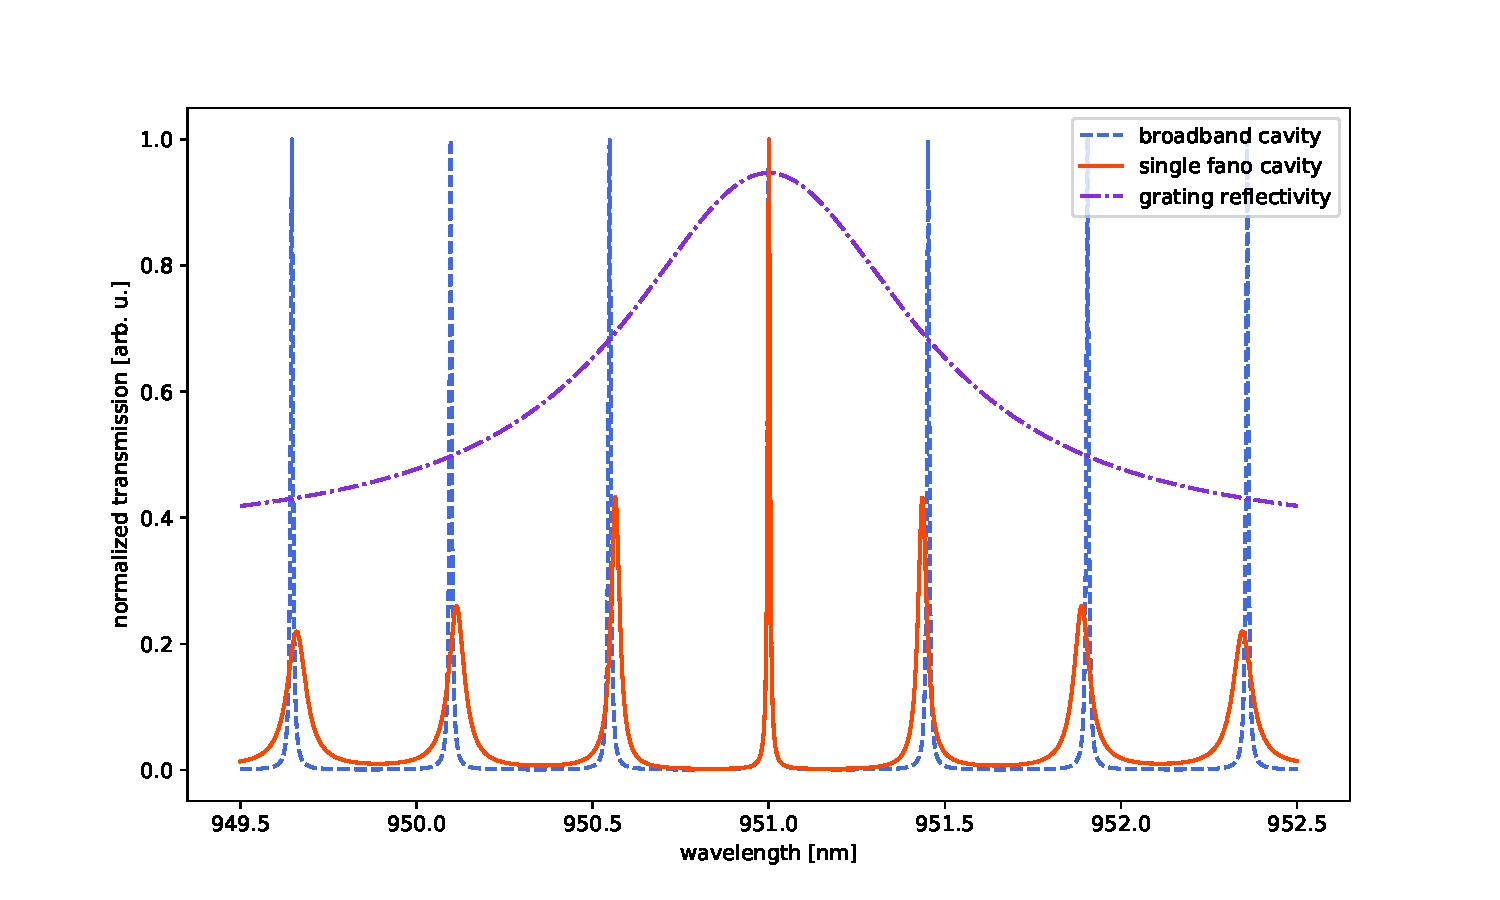
\includegraphics[width=\textwidth]{figures/fano_and_broadband_cavity_1000um.pdf}
        \caption{Broadband and single Fano transmissions for a cavity length of $\sim 1000 \mu m$, i.e. in the \emph{standard} regime.}
        \label{fig:standard_regime_trans}
    \end{subfigure}
    \begin{subfigure}[b]{0.49\textwidth}
        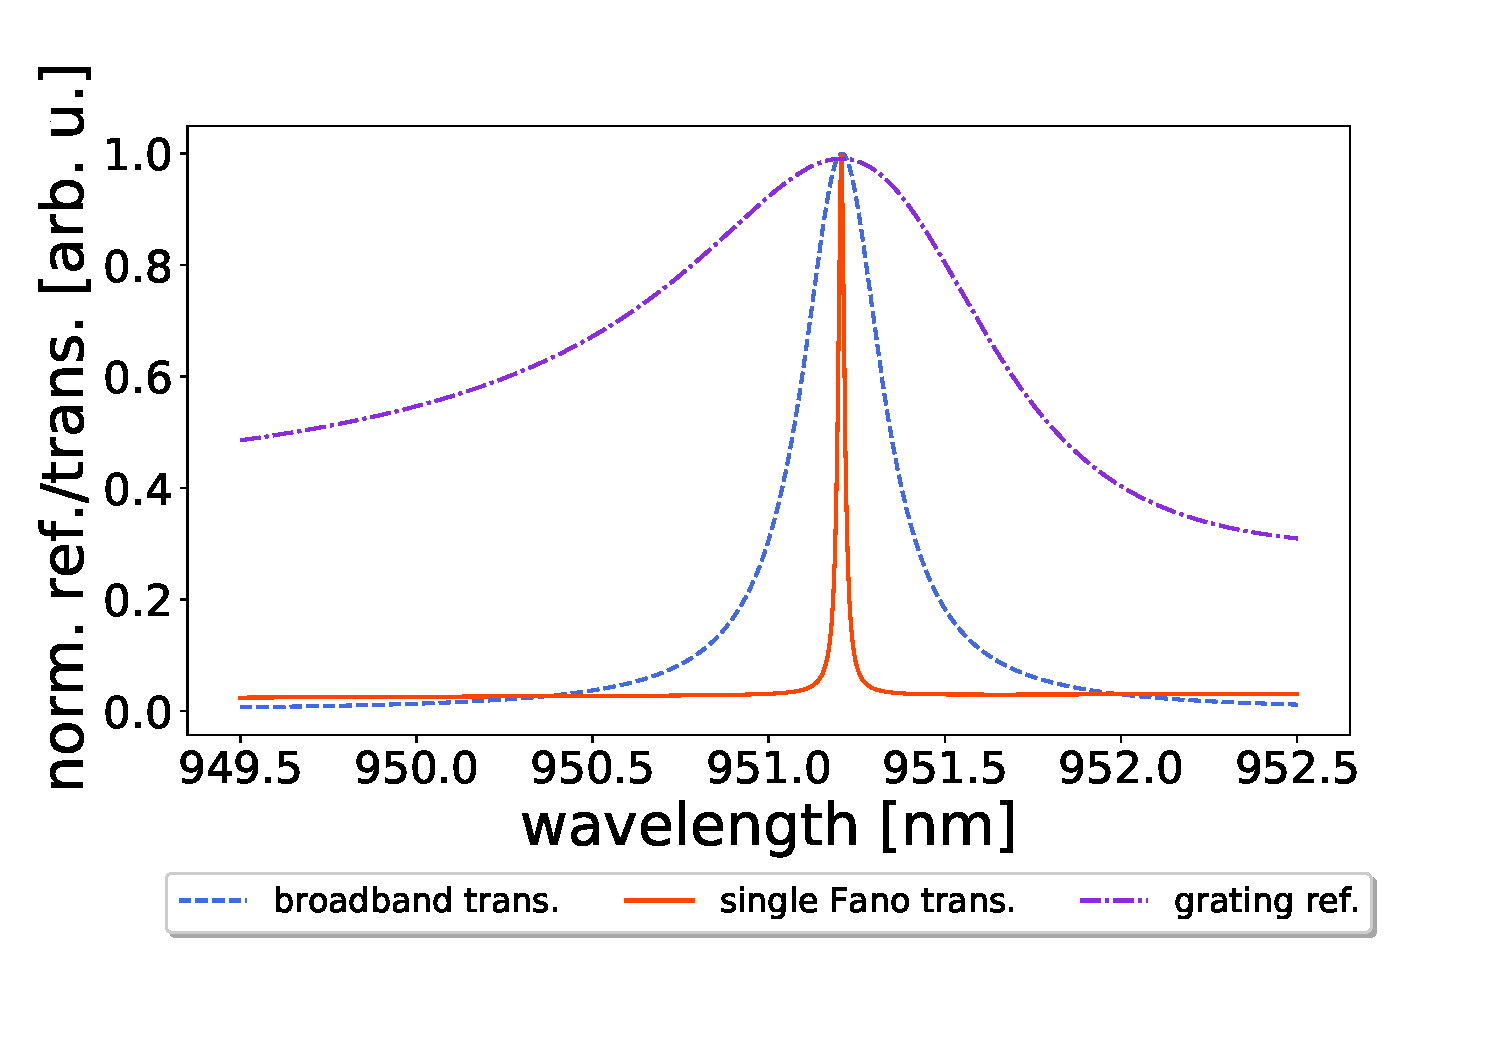
\includegraphics[width=\textwidth]{figures/fano_and_broadband_cavity_5um.pdf}
        \caption{Broadband and single Fano transmissions for a cavity length of $\sim 5 \mu m$, i.e. in the \emph{Fano} regime.}
        \label{fig:fano_regime_trans}
    \end{subfigure}
\end{figure}

Figures \ref{fig:standard_regime_trans} and \ref{fig:fano_regime_trans} depicts two examples of single Fano cavity transmission spectra together with their respective complimentary broadband cavity transmission profiles, and the reflectiviy amplitude of the Fano mirror used to model both profiles. As shown in section \ref{sec:fano_mirror} any Fano mirror, or grating, is described by five characterizing parameters. For the one used to model the transmission spectra in figures \ref{fig:standard_regime_trans} and \ref{fig:fano_regime_trans}  these are 
\begin{equation}
    \begin{split}
    \lambda_0 = &951 nm,\:\: \lambda_1 = 951 nm,\:\: t_d = 80\%,\\ &\gamma \lambda = 0.5 nm\: \text{ and }\: \beta = 10^{-6},
    \end{split}
\end{equation}
where we remember that $\lambda_{0,1}$ are the resonant wavelengths for, respectively, the cavity and guided-mode, $t_d$ is the direct transmission, $\gamma \lambda$ is the width of the guided-mode resonance and $\beta$ is a constant describing the losses of the grating, which here is neglected when solving the coupled differential equantions of eq. (\ref{eq:lossy couples diff. eqs.}). The broadband mirror parameters are chosen such that it perfectly resembles the transmission and reflectivity of the grating on resonance, which is arbitrarily chosen such that $|r_{m}|^2=95\%$ and $|t_{m}|^2 = 5\%$.

 
%% Write about the approximate analytical linewidth, and show the plot together with the simulated linewidths of both the single fano and broadband cavities to show the power of the approximation. Talk about the different regimes and show the figure of the 1000um spectrum and the 5um spectrum. Remember to include the parameters used to simulate the figures in this section.

It is clear from inspection of figure \ref{fig:standard_regime_trans} that the resonance transmission profile of the standard broadband cavity is not wavelength dependent, in the sense that all fringes, when cavity losses are neglected, appear to have the same high finesse $\mathcal{F}$, i.e. ratio between the FSR and HWHM. This is not the case for the Fano cavity which is, naturally, due to the wavelength dependence of the optical properties of the Fano mirror, as this causes the transmission and reflectivity to \emph{only} match those of the broadband mirror when on resonance. In figure \ref{fig:fano_regime_trans}, the transmission spectra of both cavities are shown \emph{in} the Fano regime, where it is clearly seen that while the standard cavity experiences broadening for shorter cavity lengths\footnote{This is a natural consequence of the shorter cavity as this causes the lifetime inside the cavity to fall and hense the transmission HWHM to rise. The HWHM is inversly proportional to the lifetime and goes as $\delta \lambda \propto 1/\tau$.}, this is not the case for the Fano cavity transmission peak.

\begin{figure}
    \centering
    \begin{subfigure}[c]{0.64\textwidth}
        \centering
        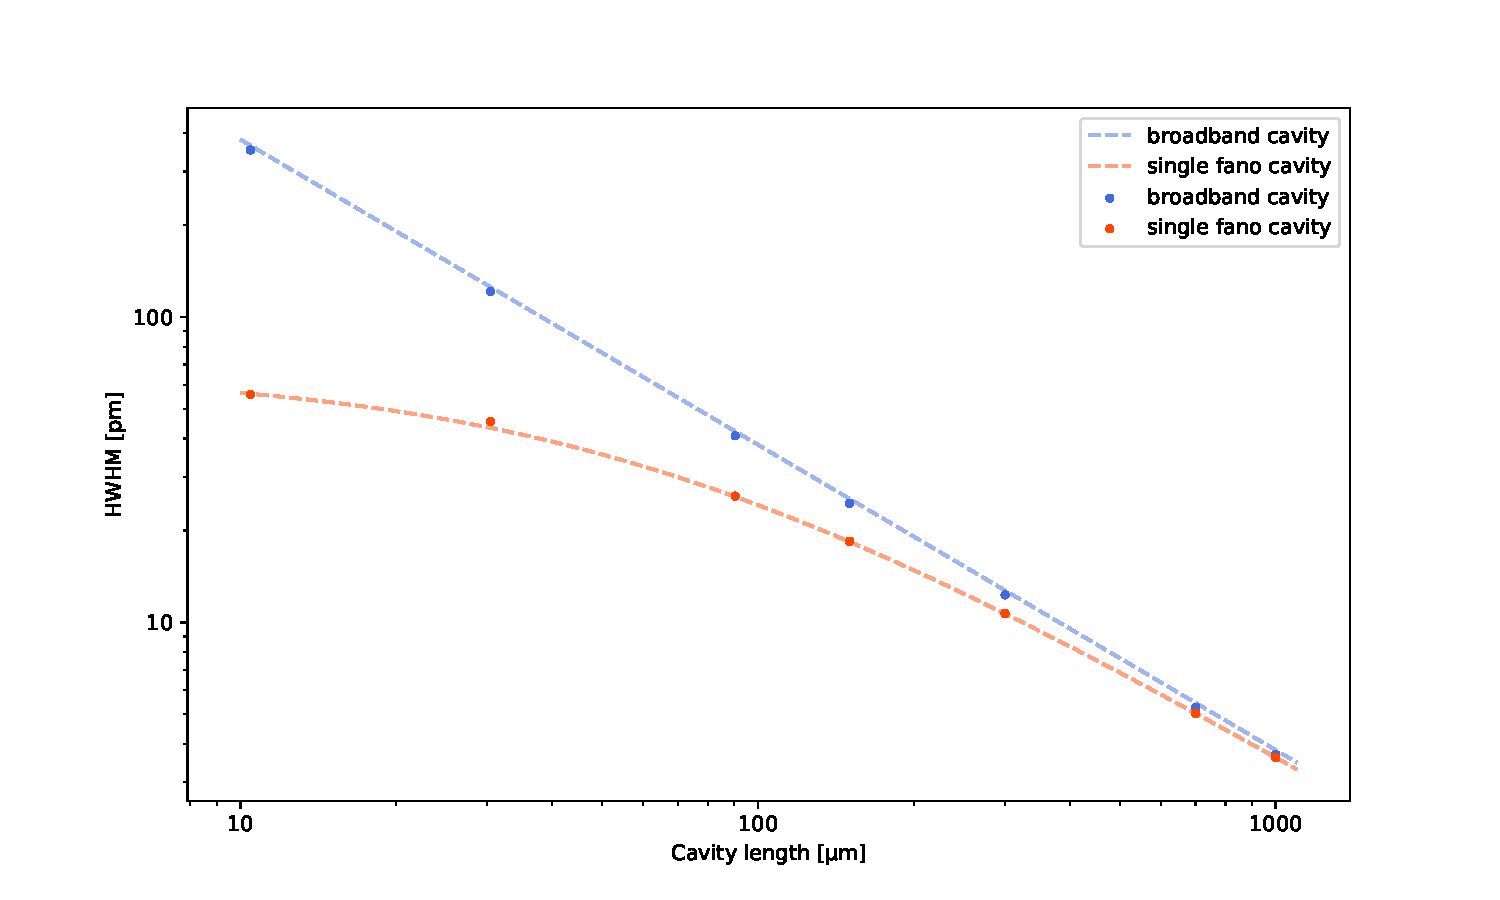
\includegraphics[width=\textwidth]{figures/HWHM_broadband_vs_single_sim.pdf}
        \caption{The approximate analytical resonance linewidths (eq. (\ref{eq:analytical_linewidth})) as a function of cavity length for the broadband and single Fano cavities are shown together with linewidths of transmission profiles simulated using eq. (\ref{eq:single_fano_trans}) and eq. (\ref{eq:fabry_perot_trans}) for comparison.}
        \label{fig:HWHM_broadband_vs_single_fano}
    \end{subfigure}
    \begin{subfigure}[c]{0.34\textwidth}
        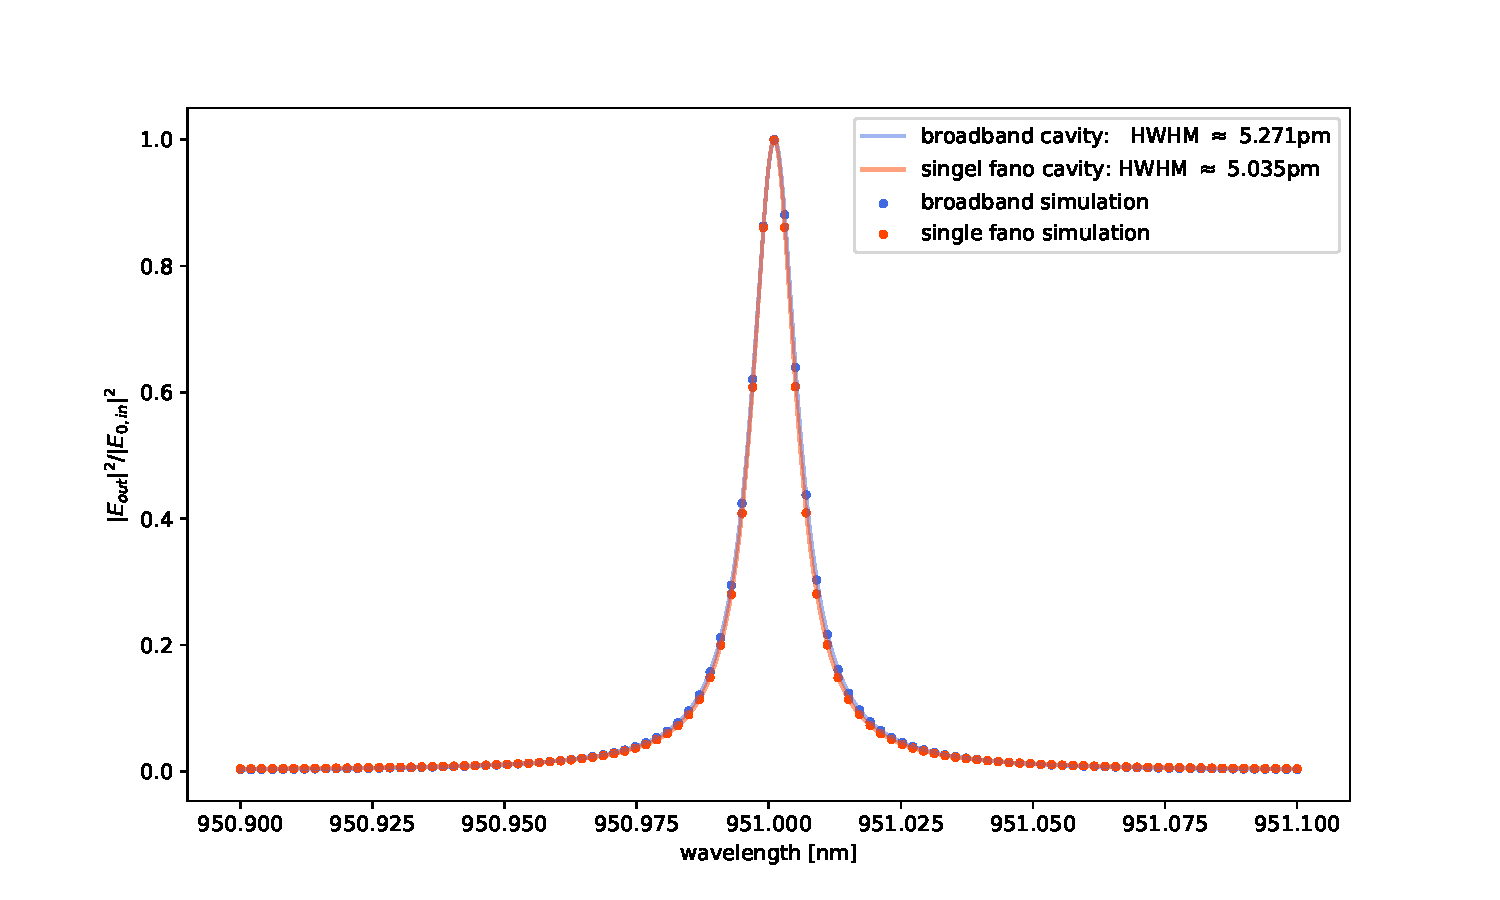
\includegraphics[width=\textwidth]{figures/sim_single_vs_broadband_700um.pdf}
        \caption{Transmission spectra of broadband and single Fano cavities of length $\sim 700 \mu m$.}
        \label{fig:700um_broadband_and_single_fano_peak}
        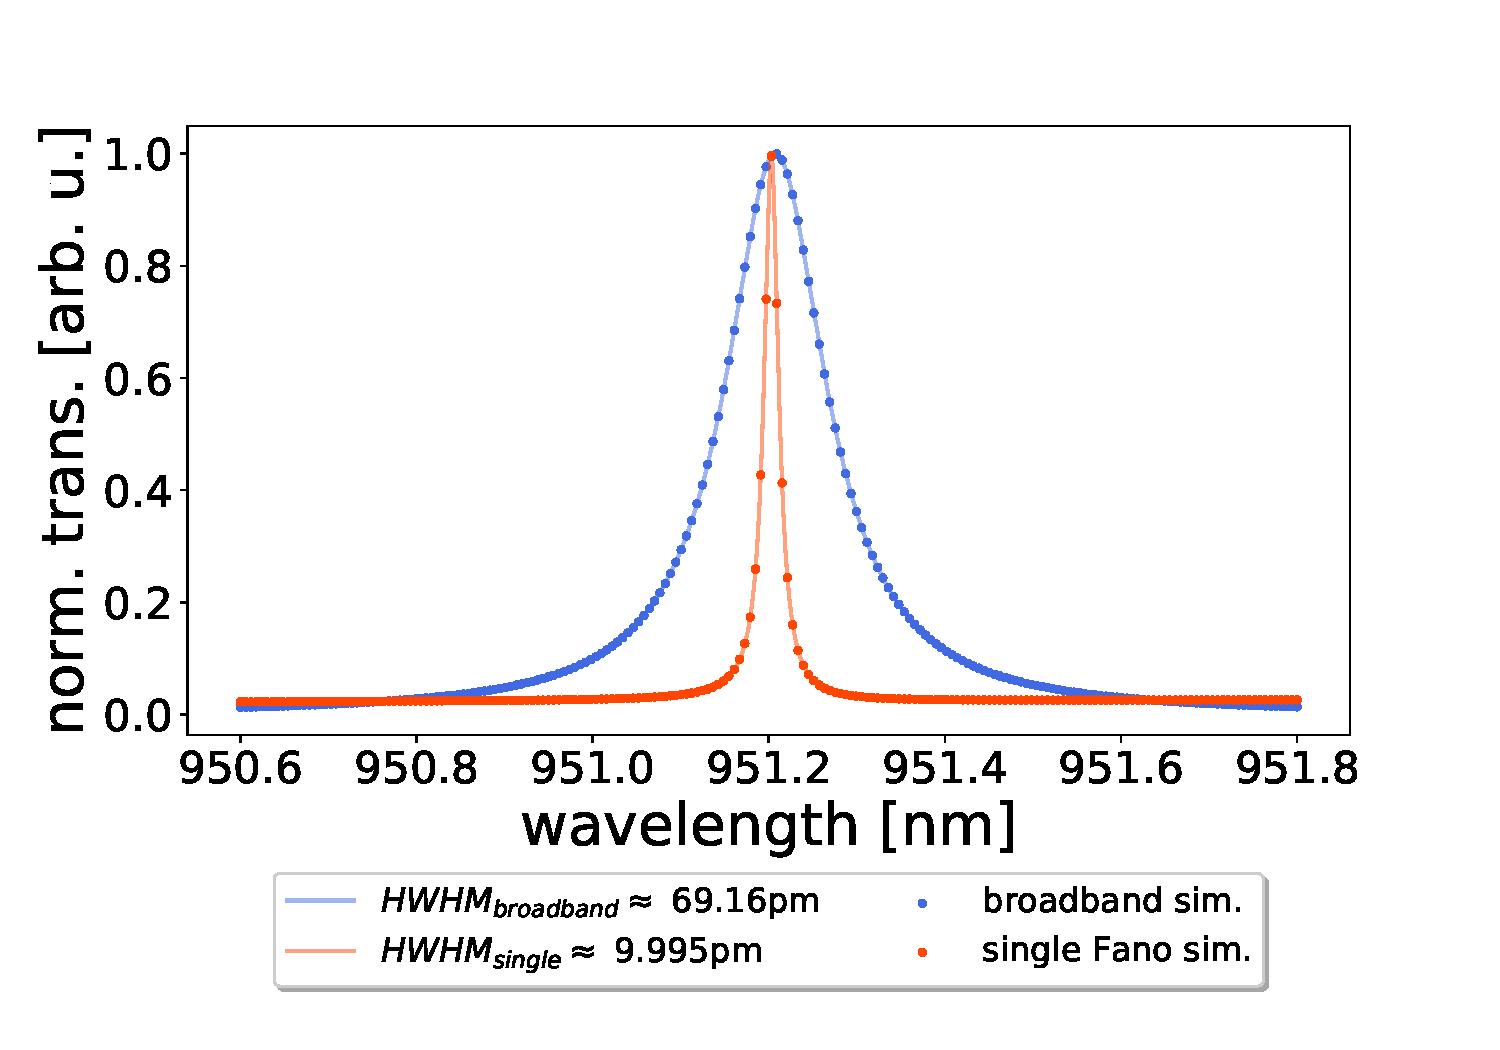
\includegraphics[width=\textwidth]{figures/sim_single_vs_broadband_10um.pdf}
        \caption{Transmission spectra of broadband and single Fano cavities of length $\sim 10 \mu m$.}
        \label{fig:10um_broadband_and_single_fano_peak}
    \end{subfigure}
\end{figure}

Figure \ref{fig:HWHM_broadband_vs_single_fano} models the behavior of the linewidth of the single Fano cavity compared with the one for a broadband cavity of similar optical properties, as a function of wavelength. Here it is easily seen where the linewidth of the single Fano begins to saturate, and hence deviate from the one of the broadband cavity. The plotted line in the figure is calculated using eq. (\ref{eq:analytical_linewidth}) while the points depicit linewidths found as a fitting parameter from a least squares fit of the general Fano model in eq. (\ref{eq:general_fano_model}) to transmission spectra simulated by the Fabry-Perot (eq. (\ref{eq:fabry_perot_trans})) and single Fano (eq. (\ref{eq:single_fano_trans})) transmission functions. Finally, it can be concluded that the approximate analytical expression for the linewidth of the broadband and single fano cavities in eq. (\ref{eq:analytical_linewidth}) correlates very well with the values found from the simulated spectra.

\subsection{The double Fano cavity: two fano mirrors}

\subsubsection{The double fano transmission model}

\subsubsection{Comparison between the double fano, single fano and broadband cavities (lossless + symmetric)}

Figures:
\begin{itemize}
    \item resonance peaks of all three cavities (maybe intracavity for easier comparison).
    \item Off-resonance trans. of all three cavities (maybe only single and double)
    \item linewidth as a function of cavity length of all three.
\end{itemize}

\subsubsection{Transmission as a function of losses (symmetric double fano cavity)}

Figures:
\begin{itemize}
    \item Trans. spectra for different values of L.
    \item linewidth as a function of L. (plot den analytiske linjebredde sammen med)
\end{itemize}

\subsubsection{Spacial and spectral detuning - $l_{g} \geq l \geq l_{g}^{\prime}$ \& $\Delta \neq 0$ (lossless double fano cavity)}

Figures (spectral detuning): 
\begin{itemize}
    \item Constructed grating trans. spectra (showing the result of varying only the spectral parameters of one grating, $\lambda_0$ and $\lambda_1$).
    \item Full range cavity transmission spectra of single + double fano cavities with grating transmission (note: resonance peak is between the trans. minima of the two gratings).
    \item Cavity trans. spectra for different values of $\Delta$ (constant cavity length).
    \item Linewidth as a function of spectral detuning $\Delta$.
\end{itemize}

Figures (spacial detuning):
\begin{itemize}
    \item Cavity trans. spectra for different lengths (small/large detuning comparison).
    \item Linewidth as a function of cavity length ($l_g \rightarrow l_g^{\prime}$).
\end{itemize}


\begin{figure}
    \centering
    \begin{subfigure}[c]{0.49\textwidth}
        \centering
        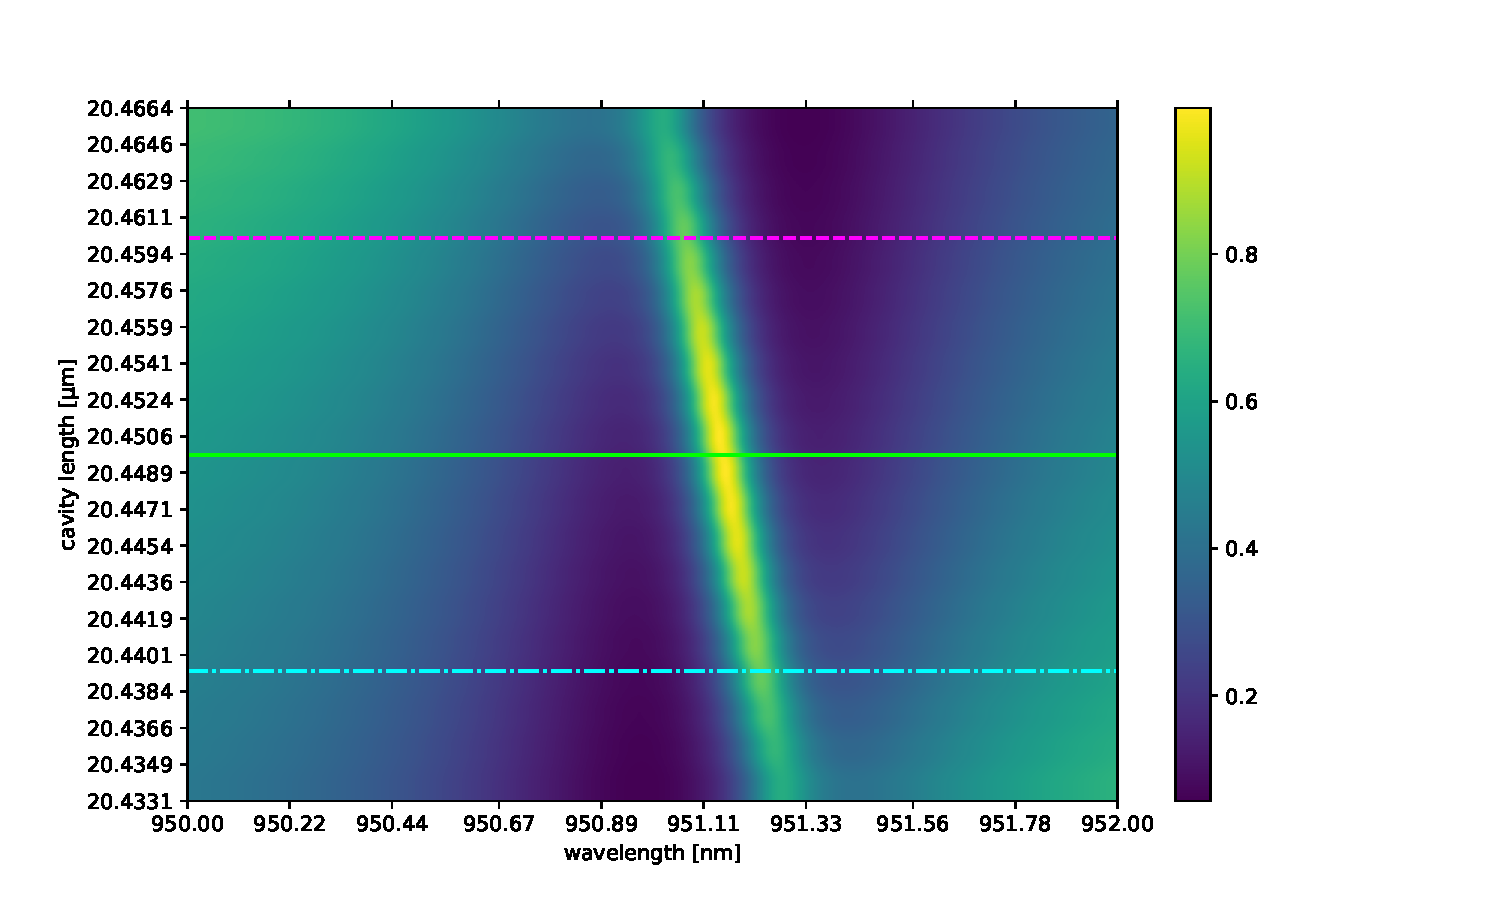
\includegraphics[width=\textwidth]{figures/cmap_with_slice_indicators1.pdf}
        \caption{cmap showing transmission as a function of wavelength for cavity lengths ranging $l_{g} \rightarrow l_{g}^{\prime}$.}
    \end{subfigure}
    \begin{subfigure}[c]{0.49\textwidth}
        \centering
        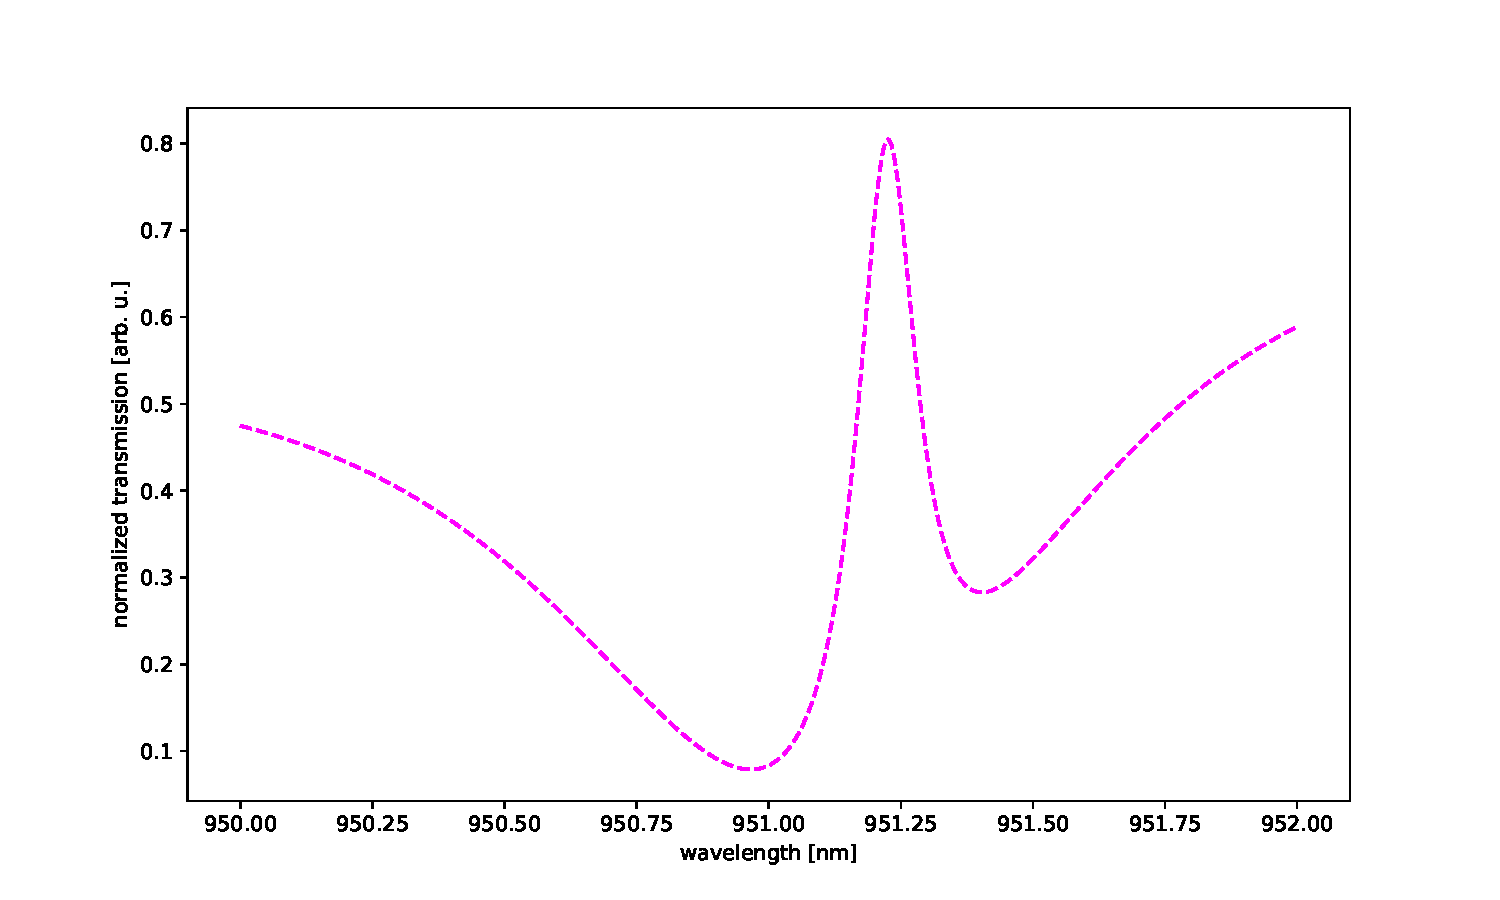
\includegraphics[width=0.49\textwidth]{figures/cmap_slice2.pdf}
        \newline
        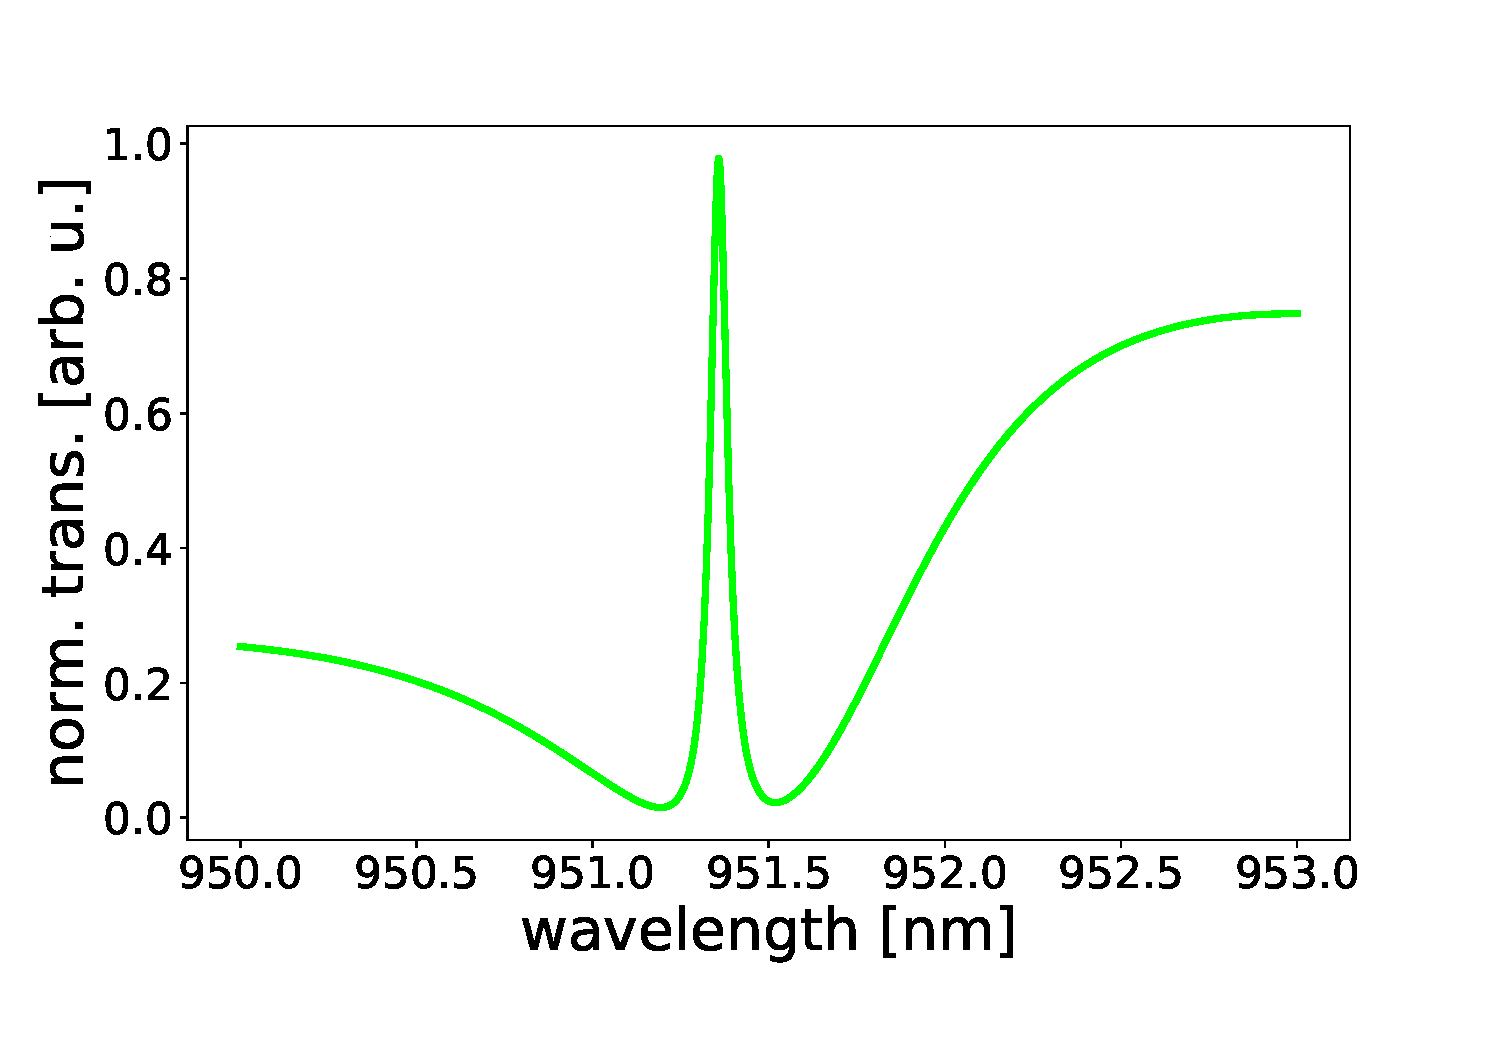
\includegraphics[width=0.49\textwidth]{figures/cmap_slice1.pdf}
        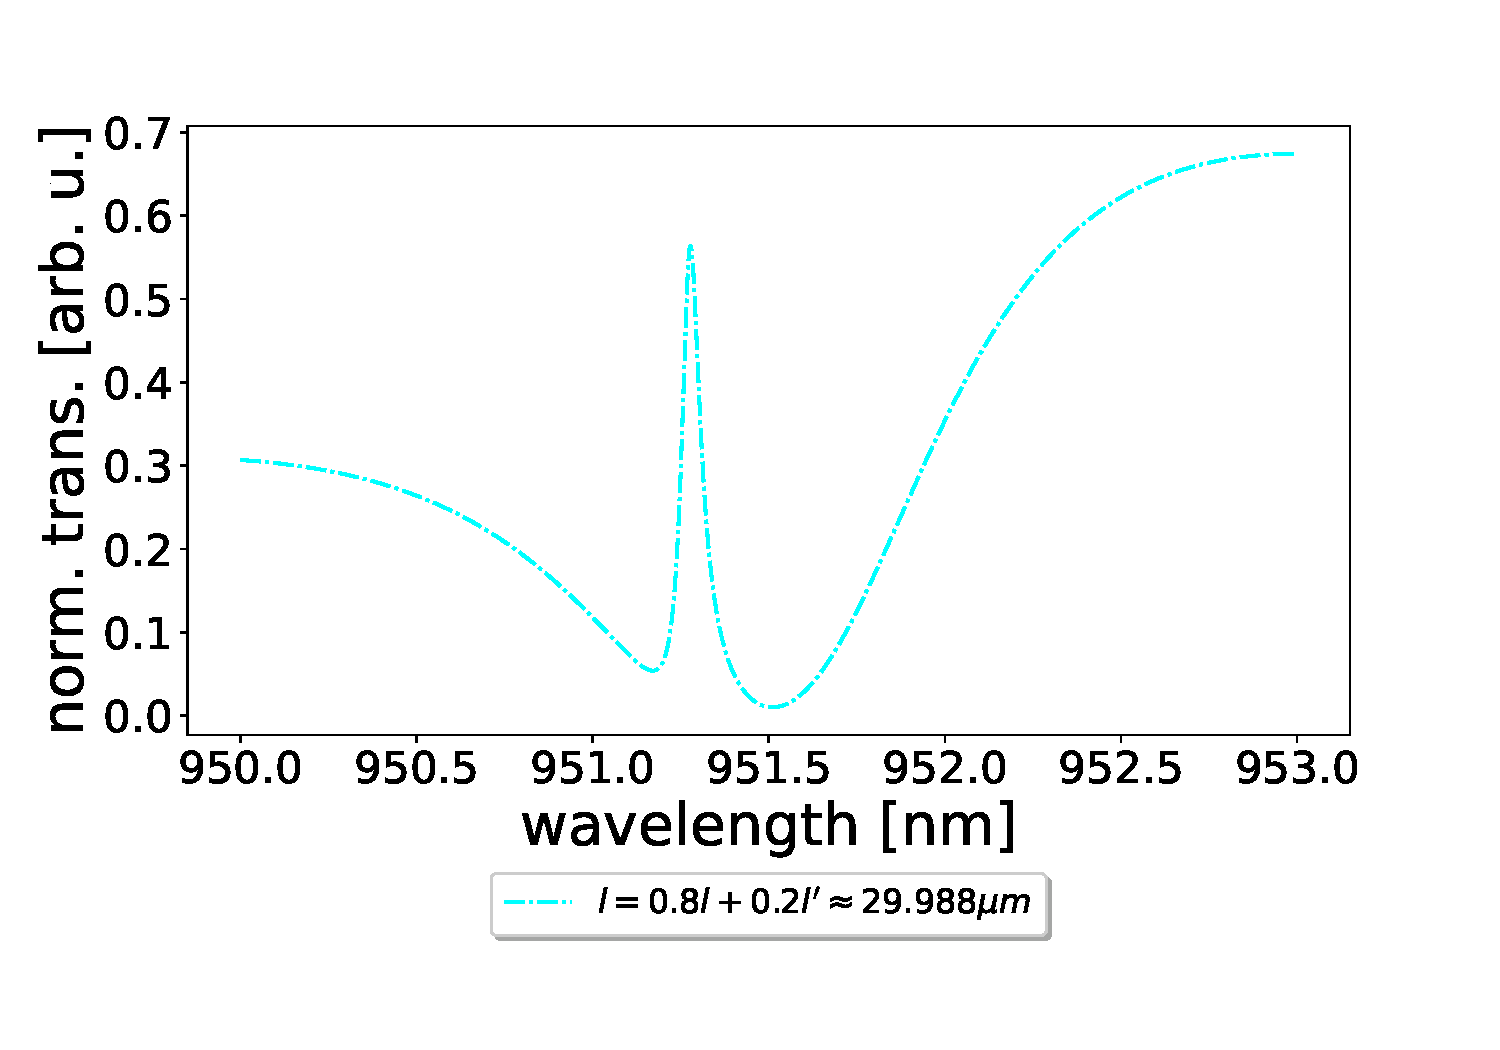
\includegraphics[width=0.49\textwidth]{figures/cmap_slice3.pdf}
        \caption{Slices of the cmap showing the optimal length and wavelength of double fano cavity (lossless). HWHMs -> Magenta = 71.3pm, cyan = 71.3pm and lime = 58.6pm.}
    \end{subfigure}
\end{figure}

\begin{figure}
    \centering
    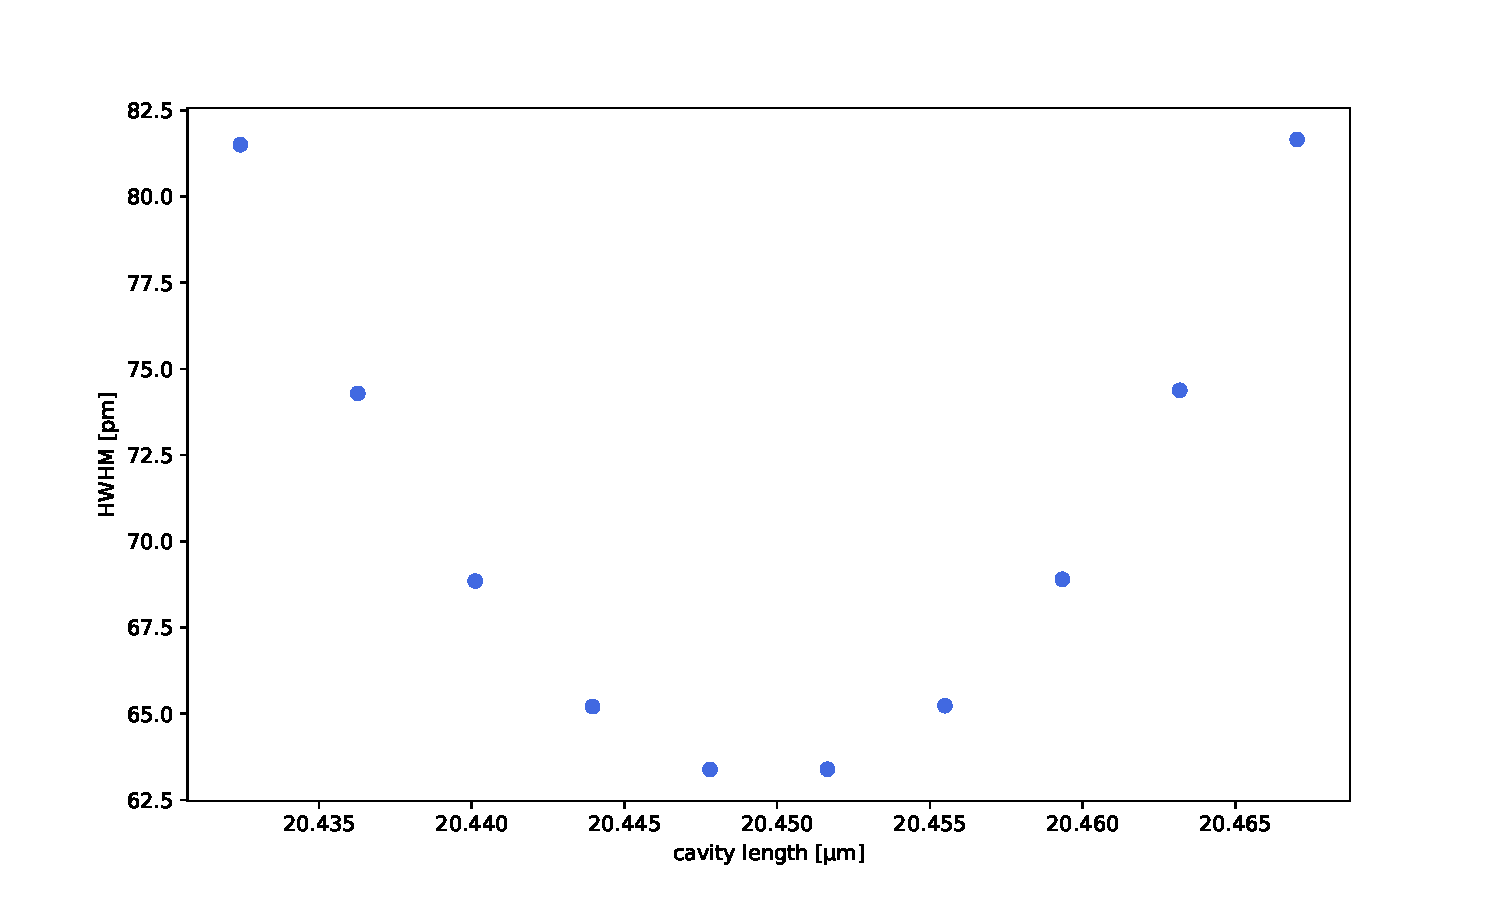
\includegraphics[width=0.5\textwidth]{figures/cmap_lw_vs_l_intracavity.pdf}
    \caption{intracavity linewidth as a function of cavity length (same cavity as depicted in cmap above.)}
\end{figure}

